\chapter{Introduction}
\section{What about it?}
The idea behind of the develop of this software isn't only to do a
useful tool for educational centers is also an excuse to research and
learn about a lot of technologies and patterns, but above all it's
about how to do clean, simple and easily readable software.
\intro
This software has been thought to help a lot of teachers in their
work, but which is exactly the problem? And how it will help?
\intro
Until a few years ago the digitalization of education was something
impossible to think, the cost of equipment and the digital illiteracy
did impossible to think in to do things of another way. The only computers
that we could see were inside the \textit{"Computer room"}, where students learned
to use a simple text processor, received simple notions of the internet
of websites, mail system or storage devices are not bad to start, but
We don't talk about this. And what about teachers? Maybe a few of
computers in some rooms or office allow them to send emails, maybe build
a simple website or offers some resource to the students (in the better case).
As we can imagine, the paper was the main support of all
about management of the center.
\intro
If we think about processes in a scholar center, we can't imagine
the amount of paper that is necessary to registry all about students,
teachers, subjects, relationships between them and the rest of work.
And the worst of this is that every three months and every year the
most of this documents, papers, records, etc. will need to redo, because
the majority of this relations will change and will be required record
all again.
\intro
Can you imagine many papers, time and effort is necessary
to do this? We will talk more about this after.
\intro
So now all people have a smartphone, the hardware is really cheap (laptops,
tablets, etc.) and open a website for an inexpert person is very
easy, and almost free, in some clicks. There are a lot of system and
tools about e-learning like Moodle\footnote{Moodle is a free and open-source
software learning management system written in PHP and distributed under the GNU
General Public License, know more at moodle.org .}, Chamilio\footnote{Chamilio is a free software
under GNU/GPL licensing e-learning and content management system backed up by
the Chamilo Association, know more at chamilio.org .} , etc that allows managing
a lot of thigs like classroom, activities, exams, etc. , all have listened sometimes about it but they have a specific domain and are
built to a specific way.
\intro
This area is more or less knowledge for the majority of new teachers
and school stuff. Many centers uses some tools like this to do a lot
of tasks, but in spite of it, there are another a lot of tools much
very heavy that is following handmade.

\section{Why to build a new tool?}

But is really necessary build to zero a new tool to do this?  Well,
if we want, could reuse some preexisting tool, maybe adding some module
to do all things that we detect that fault, but this present a lot
of problems, that are closely related to the architecture and licenses
of this software.
\intro
Because of this, is put a lot of effort in this
project in the openness of code and architecture, because this is that
make possible that the platform can  change, evolve in many
forks and feedback herself.

\section{Domain of the problem}

The idea to build SMS arises from the need of a management system for
a specific educational center in Granada that mainly speed up all
their internal management, avoid the spend of printed paper and save
huge amounts of time.
\intro
Besides this, they want a system that was helpful
for making better management decisions, in marking paths for future
improvements. To achieve that the system would need as core
a subsystem of relationships management, teachers that impart class
to students, students that are enrollments in subjects and groups
or courses, and a long etcetera. This only as the base of the system,
because with this would only be modeled the kind of relations that
the center has.
\intro
A part of this and like the minimal requirements
the center need that the system provides a simple way to do their most
heavy and paper, time and money cost, the attendance control (we can
start to see some requirements that the system would have). Appart
of this but related they need a system to save marks related with
students and disciplinary notes. Only this three things done digitally
may be a small internal revolution.

\section{The cost of non-digitalization}

Many times we do not perceive the cost of the processes in which we are involved
because we do not pay directly this cost or because we are so used to it that is
not evident.

\subsection{Paper}
How many papers are spended by a normal teacher in a high?
\intro
If we think that an ordinary teacher have 8 groups of students (if it works in a
full-time), this means 25 hours approximately at week, and each group have
25-30 student of average. In all, there are 200 students which a teacher have
relation approximately every year.
\intro
Each educational center has an own control system but normally and like in this case,
there are a lot of standard documents that each teacher manages to follow
the evolution of their students (if it does their work fine
\intro
We are going to make the calculus of these through the summary of the mainly
processes that they do.

\subsubsection{Marks and nottations}

To begin each teacher need to follow the evolution of each student in their
subject quarterly, to do this they use an official document where they write
all interesting annotations about the student, from marks of partials or final
exams to annotation about homework or class issues.
\intro
If the common teacher (here "teacher") have 200 students and in the Spanish
system we have three quarter this make up a total of 600 sheets of paper,
more another 50 by differents uses that a teacher spends commonly.
Usually, each center give to teacher a book with all these pages officially
formatted to this task, so the cost is upper that only the paper and ink.
If we multiply this number by 40 teachers approximately, we have 2400.

\subsubsection{Tutorizing}
Each time that a parent want to check the evolution of his son the mentor
of the student need to do a simple but time and money expensive process.
\intro
So, if in a medium center we have 15 mentors and each one mentoring about
30 students, and technically each of this students needs a meet with their
parents each quarter, this mean 15 * 30 * 3 * 10 subjects that the student have
 and that need an inform is equal to 9000 pages.
Including some pages necessary for the pedagogic control (parallel system of
supervision in the center).

\subsubsection{Delays}

Delays record is another process which spends paper. It is a very inefficient
whole of steps. To understand this better we are give you an example, when a
student is late (whatever the reason) a teacher need write in a officially formated
page when it was late and why (according to it).
\intro
After the student will move to another place of the center to give this paper
to an admin staff person that will
notify this to their parents (because the delay is not justified or they did not
know). This process means another 125 sheets per week between all students on average.

\subsubsection{Class attendances}

All weeks all teachers that impart class to a group write in a paper
all attendance controls of a class (independently of their own records). This
is done by all teachers. So, in on average a center have around 1000 students
and around 25 students by course, more or less 40 courses and is necessary
an attendance records paper by class, so is equal to 40 documents per week and
if the course has 32 weeks, the result is approximately 1280 sheets of paper.

\subsubsection{Another center communications}

In addition to the above, there is another kind of process in which big amounts
of paper is spent. When the direction of center wants to communicate something,
in some special days when is necessary to do this or in some activities that
simply require paper.
In the most of the cases, the excessive cost is only because there are not another better way
to do this, only for this reason. Sometimes some so easy as email or website or
simple a share document would be save a lot of money but the culture and the
dynamic of many places do difficult put into practice.


\subsubsection{Summarize}

With the follow constraint:


\begin{itemize}
  \setlength{\itemsep}{0pt}
\item A scholar course has 32 weeks at year on average (32-36 with 160-180 days).
\item The cost by printed page is about 0.03 cents of euros.
\item We are going to consider that a common center has 1000 students and 40 teachers of average.
\item More or less 25 group of students.
\item Each center has 15 mentors.
\end{itemize}

So, with this and preceding conclusion, we can obtain this costs table:

\begin{table}[H]
\centering

\begin{tabular}{@{}lllllll@{}}

Process & Per week  & Per year  & Cost  \\
\midrule

Marks and annotations   &  --  &  26000  &   780      \euro  \\
Tutorizing              &  --  &  9000   &   270      \euro  \\
Delays                  &  125 &  4000   &   120      \euro  \\
Class attendances       &  40  &  1280   &   38,4     \euro  \\
Others                  &  --  &  1000   &   30       \euro  \\

\midrule
& & & & Total & 1238,4 \euro \\
\end{tabular}
\caption{Equivalent stuff cost in managment tasks. }
\label{my-label}
\end{table}


As we can see, the cost is too much, independently of the environmental reasons.

\subsection{Time and Money}

Is not only the cost of the material resources but is also the time and their money
equivalence what we are trying to save.  If we count the hours of work that a
common teacher dedicate to do this we can estimate the cost that all student
management related work required.

\begin{table}[H]
\centering

\begin{tabular}{@{}lllllll@{}}

Stuff & Amount & Hours/Month & At year & Price Hour & Total  \\
\midrule

Teacher     & 40 & 5    & 1800 h   & 15 \euro  & 27000  \euro  \\
Admin       & 3  & 10   & 270 h   & 15 \euro  & 4050   \euro  \\
Direction   & 4  & 10   & 360 h   & 20 \euro  & 7200   \euro  \\

\midrule
& & & & Total & 38250 \euro \\
\end{tabular}
\caption{Cost based on staff work hours.}
\label{my-label}
\end{table}

\noindent This would be the cost if we think in the hours that all school stuff spend
in this kind of tasks and that have not been spent in projects of the own
center.Can you imagine many projects that would be doing with this huge
amount of houres of work by the staff of the center?
\intro
The problem is always the same, organization, control, and focused value. And
the common pattern does not have a control over all and as thinks like this,
the companies lost a lot of money and resources. The control of that happens in your
business is the most important and obviously is the only way to can take
decisions data based.
\intro
If we add the costs of the materials as paper joined to the teacher's work hours
(strictly paid), we are talking about the incredible amount of approximately
\textbf{39000 \euro} per year. A ridiculous number thinking in the cost of
software implantation.

\subsection{Value of business}

Another thing that does go unnoticed is about the values of the data that big
relational centers as school manage without any insight of their value.
In a standard center with 1000 students is generated around 10.000 records per
month, with an essential record schemas.
\intro
It is around 90.000 records per year
and if we have a more complex system with a lot of data recorded the amount can be upper.
So, what happens with all of this data. There is any value? Obviously yes,
the exploitation of this data is not very clear at first because the most of
people (centers directives included) not seen the center as a business, which
actually, it is, only that our product is the quality of the teaching that we are
offering to our students.
\intro
So, as in any manufactured process, there are a lot of steps that can be improved,
only if are controlled and measured. With students is the same (without any wrong
charm), there are a lot of steps, processes, and stages that could be improved to
offer a better education.
If we detect that by whatever reason a student have a bad trend in their evolution
is very difficult to detect if we don't have a strong system to recollect data
and be able to do a fast actuation (proactive in opposite of late traditional
reactive behavior) will be very difficult fix the problem.
\intro
And as there are a huge amount of data is difficult that anyone can process this
manually, and for this reason, is not easy too detect what part of our processes
fail or need to be improved.
All this problem can be easily solved with a powerful system that can be recollected,
processes and give human-readable way all the conclusion obtained.
\intro
And this the other big mission of the kind of software like this, offer bunisses
value of the data that help to manage.

\begin{figure}[H]
  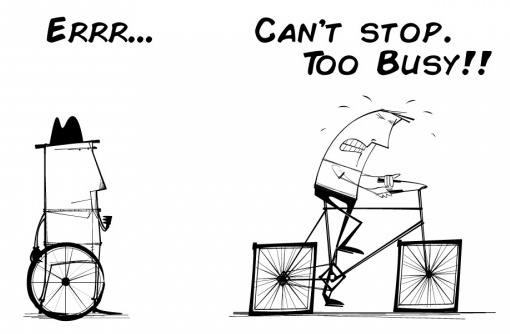
\includegraphics[scale=0.5]{img/toobusytoimprove.jpeg}
  \centering
  \caption{Too busy to improve. Author: Alan O'Rourke}
\end{figure}


\section{State of Art }

The developing of a new complete system have no sense if before have not been
analyzed other existent solutions. As part of the research process has been
analyzed some applications that (although is not a direct competition) represent
the actual state of the art about the kind of software we are talking about.
\intro
First, we take a look at the main features that are important in our domain
to see how many applications have covered them. These are a few requirements
analysis but not very formal, we will discuss about this after.
\intro
In the following table, we are going to compare the rest of app with our idyllic
software (with the features we hope it will cover).

\begin{table}[H]
\centering

\begin{tabular}{@{}lllllll@{}}

Feature & classDojo & TeacherKit & A+ & iDoceo & Additio & SMS \\ \midrule
Attendance & \completeValue & \completeValue & \completeValue & \completeValue & \completeValue & \completeValue \\
Discipline & \partialValue & \completeValue & \completeValue & \completeValue & \completeValue & \completeValue \\
Attitude & \partialValue & \completeValue & \completeValue & \completeValue & \completeValue & \completeValue \\
Marks & \noneValue & \completeValue & \completeValue & \completeValue & \completeValue & \completeValue \\
Competencias & \noneValue & \noneValue & \noneValue & \completeValue & \completeValue & \completeValue \\
Rubrics & \noneValue & \noneValue & \noneValue & \completeValue & \completeValue & \completeValue \\
Message & \completeValue & \completeValue & \completeValue & \noneValue & \noneValue &	\completeValue \\
patters & \noneValue & \noneValue & \noneValue & \completeValue & \completeValue & \completeValue \\
reports & \noneValue & \completeValue & \completeValue & \partialValue & \completeValue & \completeValue \\
analysis & \partialValue & \completeValue & \partialValue & \partialValue & \partialValue & \completeValue \\
models and predictions & \noneValue & \noneValue & \noneValue & \noneValue & \noneValue & \completeValue \\
Centralizate and jerarqy & \noneValue & \partialValue & \noneValue & \noneValue & \noneValue & \completeValue \\ \midrule

Total & 58.3\% & 80.5\% & 72.2\% & 	72.2\% & 80.5\% & 99\% \\
\end{tabular}
\caption{Features}
\label{my-label}
\end{table}

\noindent As we can see, there are some apps that are so focused on their specific domain
that is very deficient in the rest. In spite of this are referents in
their area, and their numbers of users are huge (only have been compared apps
that have a good acceptance by users).
\intro
But is not only important the features of the software, because with time and
effort any feature can be added. There are other things in the background that
are really important too and that can be that to grow our app steadily or that crash
when we have thousand of users. We are talking about something as data control,
performance, scalability or centralización (we do not explain in detail each one because
is out of his work but we think is also very important).
And of course, all related to interface and user experience, that in most of
cases can represent the difference between the successful and failure of our
project.
\intro
So, based on it this is our comparative:



\begin{table}[H]
\centering

\begin{tabular}{@{}lllllll@{}}

Feature & classDojo & TeacherKit & A+ & iDoceo & Additio & SMS \\ \midrule
Personalization & \noneValue & \noneValue & \noneValue & \noneValue & \noneValue & \noneValue \\
UI & \partialValue & \completeValue & \completeValue & \completeValue & \completeValue & \completeValue \\
UX & \partialValue & \completeValue & \completeValue & \completeValue & \completeValue & \completeValue \\
Price & \noneValue & \completeValue & \completeValue & \completeValue & \completeValue & \completeValue \\
Performance & \noneValue & \noneValue & \noneValue	 & \completeValue & \completeValue & \textcolor{ownGreen}{\completeValue} \\
Scalability & \noneValue & \noneValue & \noneValue & \completeValue & \completeValue & \completeValue \\
Data control & \completeValue & \completeValue & \completeValue & \noneValue & \partialValue & \completeValue \\
Multiplatform & \noneValue & \noneValue & \noneValue & \completeValue & \completeValue & \completeValue \\
Centralization & \noneValue & \completeValue & \completeValue & \partialValue & \completeValue & \completeValue \\ \midrule

Total & 44.4\% & 50.0\% & 16.6\% & 	16.6\% & 44.4\% & 99\% \\
\end{tabular}
\caption{Architecture and design}
\label{my-label}
\end{table}

\noindent Obviously, only in the hypothetical case of our app is fully developed will cover
all the aspects considered, but before of the research is easy to understand that
is not so difficult cover all with the correct design, architecture or design.
\intro
And we are going to try to give a simple and really little approximation of the way
to achieve that.
\intro
So, \textbf{let's start!}
